\documentclass[a4paper, 14pt]{report}
\usepackage[utf8]{inputenc}
\usepackage[russian]{babel}
\usepackage{graphicx}
\usepackage{listings}
\usepackage{color}
\usepackage{amsmath}
\usepackage{pgfplots}
\usepackage{url}
\usepackage{tikz}
\usepackage{float}

\usepackage{titlesec}
\titleformat{\chapter}[hang]{\LARGE\bfseries}{\thechapter{.} }{0pt}{\LARGE\bfseries}
\titleformat*{\section}{\Large\bfseries}
\titleformat*{\subsection}{\large\bfseries}


\lstset{ 
language=c++,                
basicstyle=\small\sffamily, 
numbers=left,  
numberstyle=\tiny,
stepnumber=1, 
numbersep=5pt,
showspaces=false, 
showstringspaces=false,
showtabs=false, 
frame=single, 
tabsize=2,  
captionpos=t, 
breaklines=true, 
breakatwhitespace=false, 
escapeinside={\#*}{*)} 
}

\usepackage{geometry}
\geometry{left=3cm}
\geometry{right=1cm}
\geometry{top=2cm}
\geometry{bottom=2cm}

\newgeometry{pdftex, left=2cm, right=2cm, top=2.5cm, bottom=2.5cm}

\begin{document}

	\begin{titlepage}
	\fontsize{12pt}{12pt}\selectfont
	\noindent \begin{minipage}{0.15\textwidth}
		
\includegraphics[width=\linewidth]{img/b_logo.jpg}
	\end{minipage}
	\noindent\begin{minipage}{0.9\textwidth}\centering
		\textbf{Министерство науки и высшего образования Российской Федерации}\\
		\textbf{Федеральное государственное бюджетное образовательное учреждение высшего образования}\\
		\textbf{«Московский государственный технический университет имени Н.Э.~Баумана}\\
		\textbf{(национальный исследовательский университет)»}\\
		\textbf{(МГТУ им. Н.Э.~Баумана)}
	\end{minipage}
	
	\noindent\rule{18cm}{3pt}
	\newline\newline
	\noindent ФАКУЛЬТЕТ $\underline{\text{«Информатика и системы управления»}}$ \newline\newline
	\noindent КАФЕДРА $\underline{\text{«Программное обеспечение ЭВМ и информационные технологии»}}$\newline\newline\newline\newline\newline\newline\newline
	
	
	\begin{center}
		\Large\textbf{Рубежный контроль №1}\newline
		\Large\textbf{по курсу "Анализ алгоритмов"}\newline
	\end{center}
	
	\noindent\textbf{Тема} $\underline{\text{~Реализация в параллельном режиме поиска подстроки в строке по алгоритму КМП}}$\newline\newline\newline
	\noindent\textbf{Студент} $\underline{\text{~~~~~Воякин А. Я.~~~~~~~~~~~~~~~~~~~~~~~~~~~~~~~~~~~~~~~~~~~~~~~~~~}}$\newline\newline
	\noindent\textbf{Группа} $\underline{\text{~~~~~ИУ7-54Б~~~~~~~~~~~~~~~~~~~~~~~~~~~~~~~~~~~~~~~~~~~~~~~~~~~~~~~~~~}}$\newline\newline
	\noindent\textbf{Оценка (баллы)} $\underline{\text{~~~~~~~~~~~~~~~~~~~~~~~~~~~~~~~~~~~~~~~~~~~~~~~~~~~~~~~~~~~~~}}$\newline\newline
	\noindent\textbf{Преподаватели} $\underline{\text{~~~~~Волкова Л.Л., Строганов Ю.В.~~~~~~~~~~~~~~~}}$\newline
	
	\begin{center}
		\vfill
		Москва~---~\the\year
		~г.
	\end{center}

\end{titlepage}
	
	\setcounter{page}{2}
	\tableofcontents
	


\newpage
\chapter{Аналитическая часть}
В данном разделе приведено описание алгоритмов поиска подстроки.

\section {Задача поиска подстроки в строке} 

Пусть дана некоторая строка T (текст) и подстрока S (слово). Задача поиска подстроки сводится к поиску вхождения этой подстроки в указанной строке. Строго задача формулируется следующим образом: пусть задан массив T из N элементов и массив S из M элементов, $0<M\leq N$. Если алгоритм поиска подстроки обнаруживает вхождение W в T, то возвращается индекс, указывающий на первое совпадение подстроки со строкой.

\section {Алгоритм Кнута-Морриса-Пратта} 

Алгоритм Кнута-Морриса-Пратта позволяет улучшить показатель количества сравнений: данный алгоритм требует только N сравнений в худшем случае.
	Идея алгоритма в том, что при каждом несовпадении T[I] и W[J] мы сдвигаемся не на единицу, а на J, так как меньшие сдвиги не приведут к полному совпадению. К сожалению, этот алгоритм поиска дает выигрыш только тогда, когда несовпадению предшествовало некоторое число совпадений, иначе алгоритм работает как примитивный. Так как совпадения встречаются реже, чем несовпадения, выигрыш в большинстве случаев незначителен.

Алгоритм  Кнута-Морриса-Пратта  основан  на  принципе  конечного автомата.     В  этом  алгоритме  состояния  помечаются  символами,  совпадение  с  которыми  должно  в  данный  момент  произойти.  Из каждого  состояния  имеется  два перехода:  один соответствует  успешно-му сравнению,  другой — несовпадению.
Успешное сравнение переводит нас  в  следующий  узел  автомата,  а  в  случае  несовпадения  мы  попадаемв  предыдущий  узел,   отвечающий  образцу.

При  всяком  переходе  по  успешному  сравнению  в  конечном  автомате Кнута-Морриса-Пратта  происходит  выборка  нового  символа  из  текста.   Переходы,  отвечающие  неудачному  сравнению,  не  приводят  к  выборке  нового  символа;  вместо  этого  они  повторно  используют  последний выбранный  символ.  Если  мы перешли  в  конечное состояние,  то это означает,  что  искомая  подстрока  найдена.

Заметим,  что  при  совпадении  ничего  особенного  делать  не  надо:  происходит  переход  к  следующему  узлу. Напротив,  переходы  по  несовпадению  определяются  тем,  как  искомая подстрока соотносится  сама  с  собой.

Метод КМП использует предобработку искомой строки, а именно: на ее основе создается префикс-функция.
Префикс-функция от строки $S$ и позиции $i$ в ней — длина $k$  наибольшего собственного (не равного всей подстроке) префикса подстроки $S[1.. i]$, который одновременно является суффиксом этой подстроки.
То есть, в начале подстроки $S[1.. i]$ длины $i$ нужно найти такой префикс максимальной длины $k < i$, который был бы суффиксом данной подстроки $S[1..k]=S[(i-k+1)..i]$.

Например, для строки "abcdabscabcdabia" префикс-функция будет такой:

[0 ,0 ,0 ,0 ,1 ,2 ,0 ,0 ,1 ,2 ,3 ,4 ,5 ,6 ,0 ,1].

Значения префикс-фукнции для каждого символа шаблона вычисляются перед началом поиска подстроки в строке и затем используются для сдвига.
	
	Особенностью данного алгоритма является то, что он работает на основе автоматов. 
	

	\section{Вывод}
	Были рассмотрены три различных алгоритма поиска подстроки в строке.
	
	\newpage
	\chapter{Конструкторская часть}
	
	В данном разделе была поставлена задача поиска подстроки в строке и описан алгоритм КМП.
	
	\section{Схемы алгоритмов}
	
	На рис. \ref{fig:kmp} представлена схема алгоритма Кнута-Морриса-Пратта:
    
    \begin{figure}[H]
        	\begin{center}
        		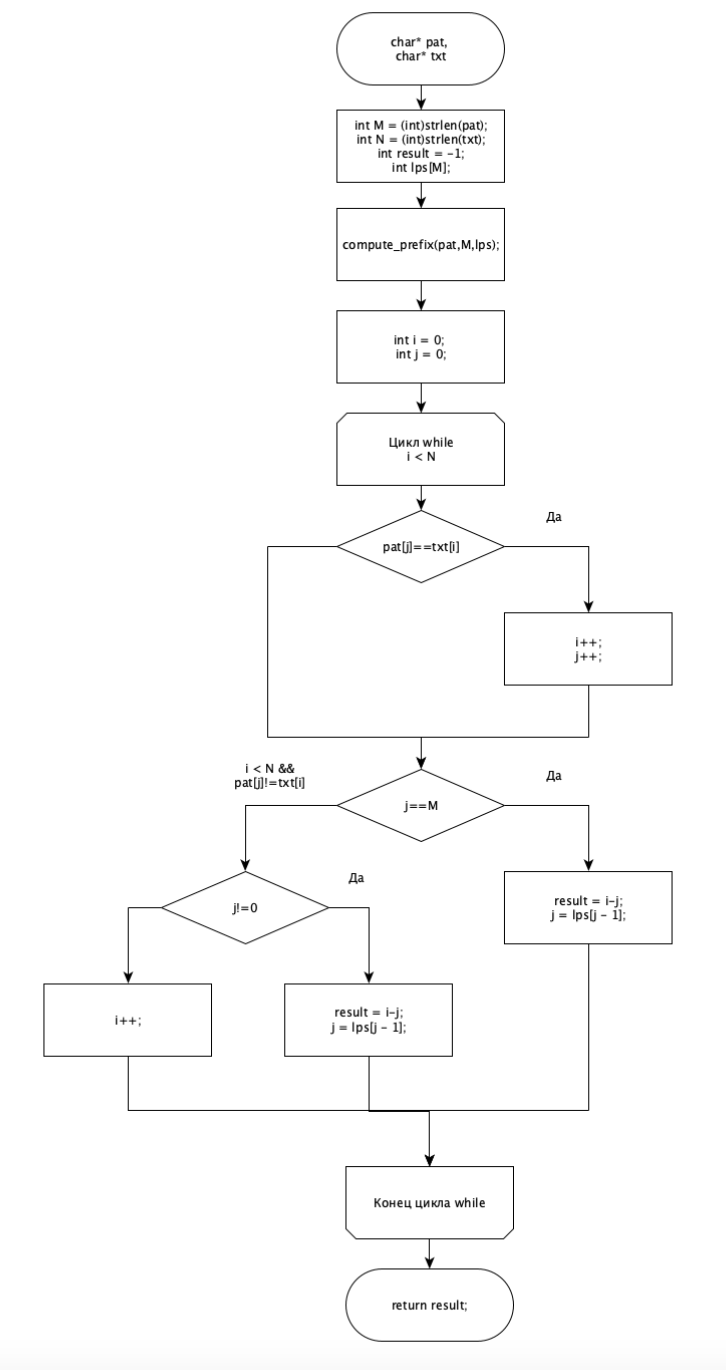
\includegraphics[scale=0.65]{img/kmp.png}
        		\caption{Схема алгоритма Кнута-Морриса-Пратта}
        		\label{fig:kmp}
        	\end{center}
        \end{figure}
\newpage
        На рис. \ref{fig:pref} представлена схема алгоритма нахождения префикса:
    
    \begin{figure}[H]
        	\begin{center}
        		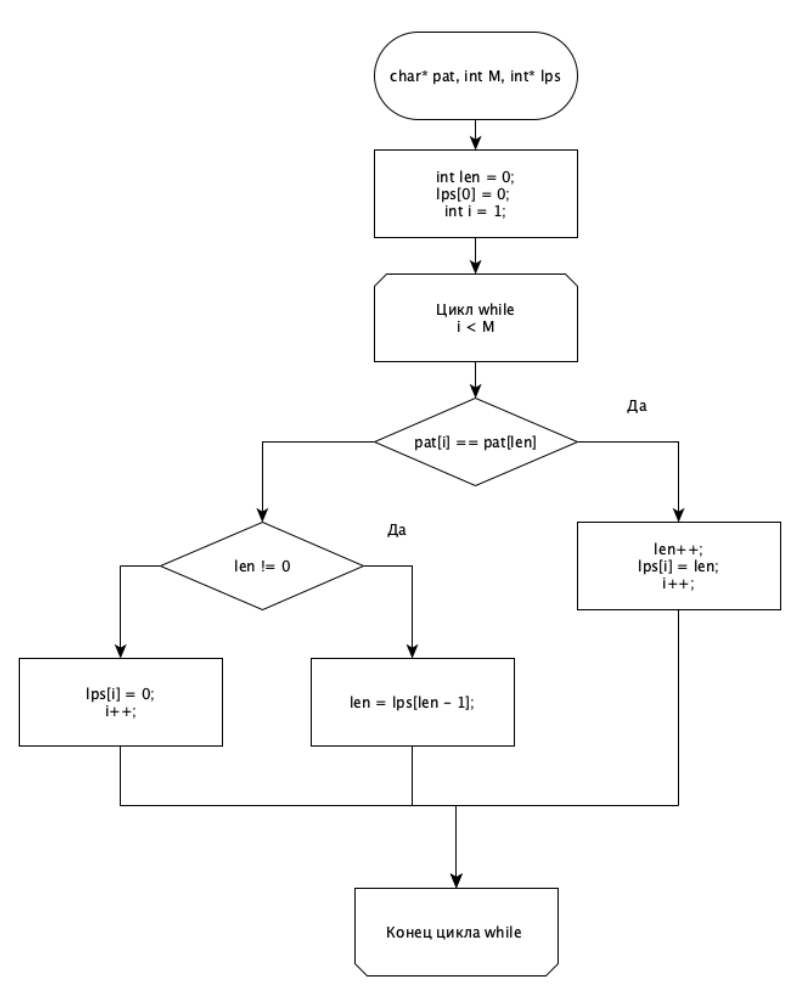
\includegraphics[scale=0.9]{img/pref.png}
        		\caption{Схема алгоритма нахождения префикса}
        		\label{fig:pref}
        	\end{center}
        \end{figure}
       

	\section{Вывод}
	
	В данном разделе были рассмотрены схемы алгоритмов.

	\newpage
	\chapter{Технологическая часть}
	
	В этом разделе будут изложены требования к программному обеспечению и листинги алгоритмов.
	
	\section{Средства реализации}
	
		Данная программа разработана на языке C++, поддерживаемом многими операционными системами. Проект выполнен в среде Xcode. \\
	
\section{Листинги функций}

В данном разделе представлен листинг реализованного алгоритма.\\

В листинге \ref{kmp_parallel} представлен распараллеленный алгоритм Кнута-Морриса-Пратта.\\



\begin{lstlisting}[label=kmp_parallel,caption=Распараллеленный алгоритм Кнута-Морриса-Пратта]
static vector<string> mainFunc(vector<string> patterns, vector<string> text, const int threads) {
	vector<string> result;
	size_t numberOfStrings = text.size(); 
	
	omp_set_num_threads(threads);
	#pragma omp parallel for num_threads(threads) 
	for (int i = 0; i < numberOfStrings; i++) {
		for (int j = 0; j < patterns.size(); j++) {
			string resultOfLine = "";
			if (text[j] == "") continue;
			KMP(patterns[j], text[i], resultOfLine);
			if (!resultOfLine.empty()) {
				string numberLine = "\n\t Pattern \"" + patterns[j] + "\", number of line: " + to_string(i + 1);
				#pragma omp critical 
				{
					result.push_back(numberLine);
					result.push_back(resultOfLine);
					result.push_back(text[i]);
				}
			}
		}
	}
	return result;
}

static vector<int> ComputePrefixFunction(string P) {
	size_t len = P.length();
	vector<int> s;
	for (int i = 0; i < len; i++) s.push_back(0);
	int border = 0;
	for (int i = 1; i < len; i++) {
		while ((border > 0) && (P[i] != P[border])) {
			int index = border - 1;
			border = s[index];
		}
		if (P[i] == P[border]) border = border + 1;
		else border = 0;
		s[i] = border;
	}
	return s;
}

static vector<int> FindAllOccurrences(string P, string T) {
	string S = P + '#' + T;
	vector<int> s = ComputePrefixFunction(S);
	vector<int> result;
	int len_pattern = P.length();
	for (int i = (len_pattern + 1); i < S.length(); i++) {
		if (s[i] == len_pattern) {
			int find = 1 + i - 2 * len_pattern;
			result.push_back(find);
		}	
	}
	return result;
}

void KMP(string Pattern, string Text, string &result) {
	vector<int> res = FindAllOccurrences(Pattern, Text);
	int len = Pattern.length();
	for (int i = 0; i < res.size(); i++) {
		int start = res[i];
		int end = start + len - 1;
		string buffer = "   " + to_string(start) + "-" + to_string(end);
		result += buffer;
	}
} 
\end{lstlisting}
	

	\section{Вывод}

В данном разделе были представлены листинги реализованных алгоритмов.

\newpage
	\chapter{Исследовательская часть}
	В данном разделе будут приведены примеры работы программы.\\

	\section{Примеры работы}
	
На рисунке 4.1 представлена демонстрация работы программы:
	
	\begin{figure}[H]
        	\begin{center}
        		{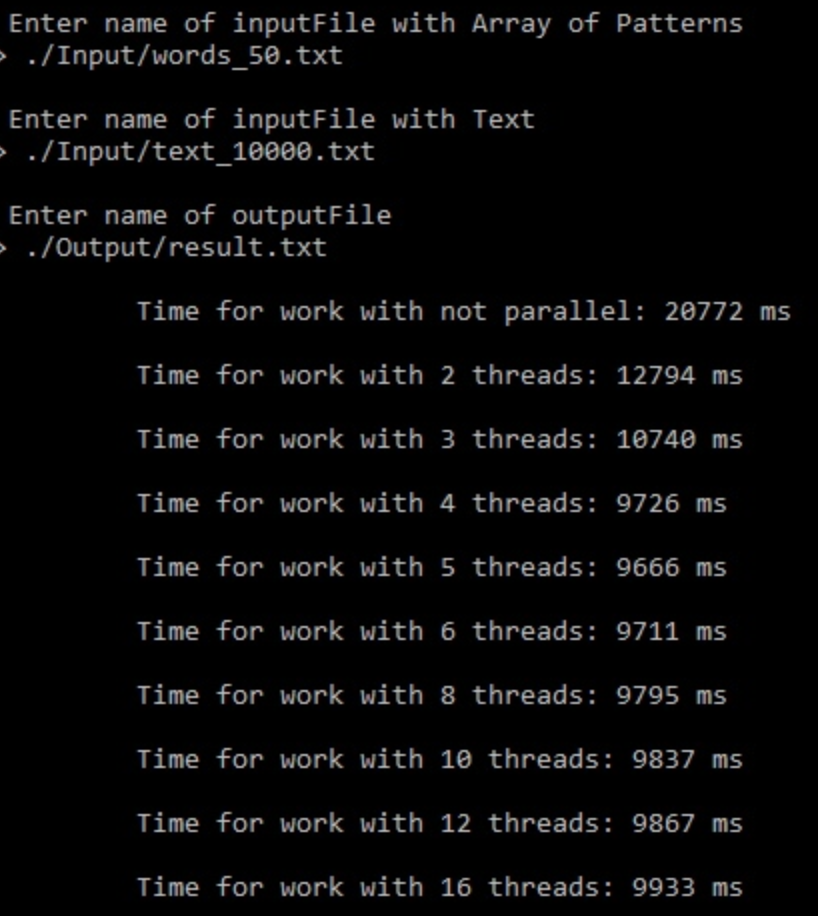
\includegraphics[scale = 0.7]{img/example.png}}
        		\caption{Демонстрация работы программы}
        	\end{center}
        \end{figure}



	\section{Вывод}
	
	В данном разделе были приведены примеры работы программы.

	\newpage
	\section*{Заключение}
	
	\addcontentsline{toc}{section}{Заключение}
	В ходе выполнения был реализован в параллельном режиме поиск подстроки в строке по алгоритму КМП.
	
\newpage
\addcontentsline{toc}{section}{Список  литературы}

\begin{thebibliography}{}
    \bibitem{litlink1}  Дж. Макконнелл. Анализ алгоритмов. Активный обучающий подход.-М.:Техносфера, 2009.
\end{thebibliography}
	
	\newpage
	\bibliographystyle{alpha}
	\bibliography{mybib}
	
\end{document}
